% visualization.tex — \input'd from experiments/experiments.tex
%
% Sources: experiments/visualization/ (Three.js interactive viewer),
%   crates/src/geom/reeb_trajectory.rs (trajectory simulation).
%
% Math claims requiring Jörn's verification:
%   - Stereographic projection formula (Eq. \ref{eq:stereo-proj})
%   - Reeb vector formula R_i = (2/h_i) J_0 n_i and tangency of J_0 n_i
%   - Conformality of stereographic projection (stated without proof)

\subsection{Visualization of Reeb Dynamics}
\label{sec:visualization}

To build geometric intuition about Reeb flows on polytope boundaries,
we visualize $\mathbb{R}^4$ polytopes and their Reeb trajectories via
stereographic projection to~$\mathbb{R}^3$.

\subsubsection*{Projection pipeline}

The visualization uses a two-stage projection:
\[
  \partial K \;\xrightarrow{\;\text{radial}\;}\; S^3
  \;\xrightarrow{\;\text{stereographic}\;}\; \mathbb{R}^3.
\]

\emph{Radial projection.}
The map $x \mapsto x / \lVert x \rVert$ sends $\partial K$ to~$S^3$.
This is well-defined since $K$ is a convex body containing the origin
in its interior, so every ray from the origin meets $\partial K$
exactly once.

\emph{Stereographic projection.}
We use stereographic projection because it is conformal
(preserving angles locally) and maps great circles on~$S^3$
to circles or lines in~$\mathbb{R}^3$, so the polytope's
combinatorial structure remains visually recognizable.
Fix a north pole $n \in S^3$. For $y \in S^3 \setminus \{n\}$,
the stereographic projection sends $y$ to the intersection of the ray
from~$n$ through~$y$ with the tangent hyperplane to~$S^3$ at~$-n$.
In coordinates:
\begin{equation}
  \label{eq:stereo-proj}
  \pi_n(y) \;=\; \frac{y - \langle y, n \rangle \, n}{1 - \langle y, n \rangle},
\end{equation}
which maps $S^3 \setminus \{n\}$ conformally to~$\mathbb{R}^3$
(identified with the hyperplane $n^\perp$ via an orthonormal basis).

\emph{Pole singularity.}
Points near the north pole project to large radii.
The implementation clips geometry within an angular neighbourhood
of~$n$: a point~$y \in S^3$ is omitted when
$\langle y, n \rangle \geq (R^2 - 1)/(R^2 + 1)$,
where $R$ is a configurable clipping radius.
Line segments passing through this neighbourhood are split at the
boundary and only the exterior portions are drawn.
This produces visible gaps in edges and trajectories near the pole,
which is expected and does not indicate missing geometry.

\subsubsection*{Reeb trajectories}

On each facet~$F_i$ with outward unit normal~$n_i$ and height~$h_i$,
the Reeb vector field is $R_i = \frac{2}{h_i} J_0 \, n_i$,
where $J_0$ is the standard complex structure on~$\mathbb{R}^4$.
The direction $J_0 n_i$ is tangent to~$F_i$ since
$\langle J_0 n_i, n_i \rangle = \omega_0(n_i, n_i) = 0$
by antisymmetry of~$\omega_0$.
For visualization, we use the direction~$J_0 n_i$ only,
as the factor~$2/h_i$ rescales time but does not affect the trajectory shape.

A Reeb trajectory is simulated by forward integration:
starting at a point on a facet, follow the constant Reeb direction
until hitting a neighbouring facet (a ridge), then switch to the
new facet's Reeb vector.
This produces a piecewise-linear curve on~$\partial K$.
The simulation starts from the vertex centroid of each facet and
runs for up to 100 segments or until the trajectory closes
(returns within tolerance of its start).

\begin{figure}[ht]
\centering
\begin{minipage}{0.48\textwidth}
  \centering
  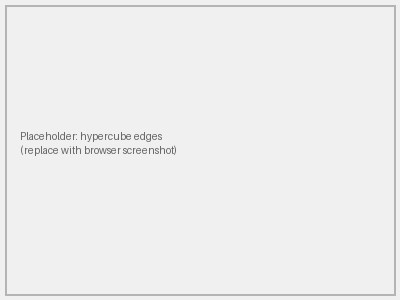
\includegraphics[width=\textwidth]{../experiments/visualization/viz-hypercube-edges.png}
\end{minipage}\hfill
\begin{minipage}{0.48\textwidth}
  \centering
  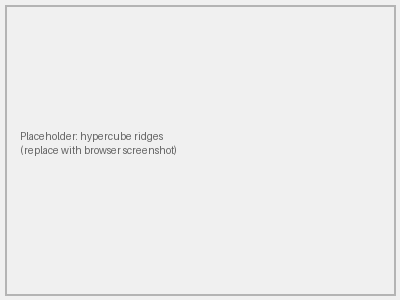
\includegraphics[width=\textwidth]{../experiments/visualization/viz-hypercube-ridges.png}
\end{minipage}
\caption{Stereographic projection of the hypercube $[-1,1]^4$
  from the north pole $n = e_4$.
  Left: vertices and edges.
  Right: ridges (2-faces), which appear as curved surfaces
  since great-circle arcs on~$S^3$ map to circles in~$\mathbb{R}^3$.}
\label{fig:viz-hypercube}
\end{figure}

\begin{figure}[ht]
\centering
\begin{minipage}{0.48\textwidth}
  \centering
  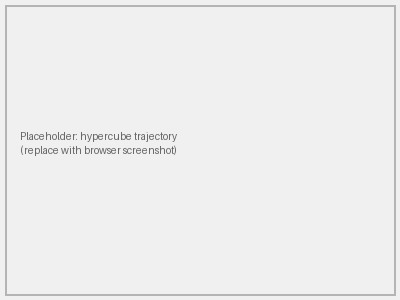
\includegraphics[width=\textwidth]{../experiments/visualization/viz-hypercube-traj.png}
\end{minipage}\hfill
\begin{minipage}{0.48\textwidth}
  \centering
  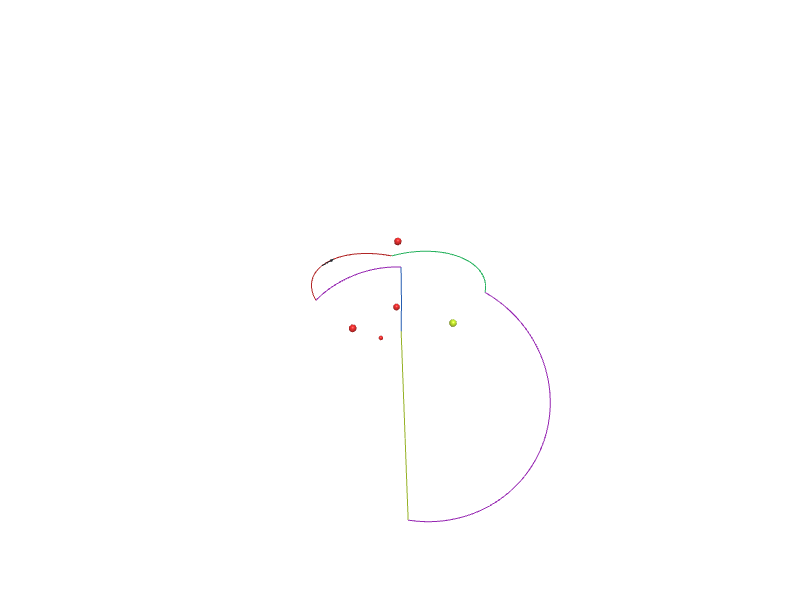
\includegraphics[width=\textwidth]{../experiments/visualization/viz-simplex-traj.png}
\end{minipage}
\caption{Single Reeb trajectories after stereographic projection
  from $n = e_4$.
  Left: hypercube, trajectory starting from facet centroid of~$F_0$,
  visiting 4 of 8 facets.
  Right: simplex, trajectory starting from facet centroid of~$F_0$,
  visiting all 5 facets.
  See Table~\ref{tab:viz-trajectories} for trajectory parameters.}
\label{fig:viz-trajectories}
\end{figure}

\subsubsection*{Observations}

The interactive visualization renders the eight known polytopes
from the dataset library and is available online at
\url{https://joernstoehler.github.io/msc-math/viz/}.
For each polytope, the user can toggle display of vertices, edges,
ridges (2-faces), and Reeb trajectories, select individual
trajectories, and rotate the stereographic north pole.
Figures~\ref{fig:viz-hypercube} and~\ref{fig:viz-trajectories}
show representative screenshots.

Several qualitative features are visible:

\begin{itemize}
  \item On the hypercube $[-1,1]^4$, trajectories visit a restricted
    subset of facets (4 of~8), reflecting the high symmetry of the
    polytope.
    The projected trajectory in Figure~\ref{fig:viz-trajectories}~(left)
    forms a compact, nearly elliptical curve.

  \item On less symmetric polytopes (e.g., the simplex with 5 facets
    or the HK-O pentagon with~10), trajectories visit all facets
    and trace more complex paths through the projected geometry.

  \item The choice of north pole affects the visual appearance
    substantially but not the underlying geometry.
    Choosing the pole along a coordinate axis direction
    tends to produce more interpretable projections.

  \item Ridges (2-faces) curve under the stereographic projection
    (Figure~\ref{fig:viz-hypercube}, right),
    giving visual evidence that great-circle arcs on~$S^3$ map to
    circles in~$\mathbb{R}^3$.
\end{itemize}

\begin{table}[ht]
\centering
\begin{tabular}{lcccc}
\toprule
Polytope & Facets & Segments & Facets visited & Start \\
\midrule
Hypercube       & 8  & 100 & 4 of 8  & centroid of $F_0$ \\
Simplex         & 5  & 100 & 5 of 5  & centroid of $F_0$ \\
HK-O pentagon   & 10 & 100 & 10 of 10 & centroid of $F_0$ \\
Crosspolytope   & 16 & 100 & 4 of 16 & centroid of $F_0$ \\
Lag.\ $\triangle$-product & 6 & 30 & 4 of 6 & centroid of $F_0$ \\
\bottomrule
\end{tabular}
\caption{Trajectory parameters for the Reeb trajectories shown in the
  interactive visualization.
  Each trajectory starts from the vertex centroid of facet~$F_0$
  and is simulated for up to 100 segments.
  None of the trajectories close within the simulation horizon.}
\label{tab:viz-trajectories}
\end{table}

\subsubsection*{Implementation}

The visualization consists of a Rust export tool
(\texttt{datasets::viz\_export}) that writes the polytope skeleton
and trajectory data as JSON, and a browser-based viewer
(\texttt{experiments/viz/}) using Three.js.
The viewer loads the JSON data and performs the projection pipeline
in JavaScript, rendering the result as an interactive 3D scene.
Sampling along edges and ridges uses spherical linear interpolation
(slerp) on~$S^3$ to produce uniform angular spacing, which
stereographic projection maps to smooth~$\mathbb{R}^3$ spacing.
